
\documentclass[a4paper]{article}
\usepackage{ngerman}
\usepackage[latin1]{inputenc}
\usepackage{a4wide}
\usepackage{graphicx}

\begin{document}

\title{Serie 10}
\author{Hannes Georg (850360), Matthias B�hm (895778) }
%\maketitle

\section*{Aufgabe 1 b)}

Berechnung der theoretischen Rundheit f�r Kreis und Quadrat: 

\begin{itemize}
\item Quadrat:

Sei a die L�nge einer Kante. Dann ist der Umfang $4a$. 
Die Fl�che des Quadrates ist dann $a^2$, und die Roundness ist
$\frac{(4a)^2}{a^2} = \frac{16a^2}{a^2} = 16$. 

\item Kreis:

Sei r der Radius des Kreises. Dann ist der Umfang $2\pi r$, und
die Fl�che ist $\pi r^2$. Dann ist die Roundness
$ \frac{(2\pi r)^2}{\pi r^2} = \frac { 4 \pi^2 r^2}{\pi r^2} 
= 4\pi \approx 12,566 $. 

\end{itemize}

Die vom Programm errechneten Rundheitswerte sind im Allgemeinen gr��er als die theoretischen Rundheitswerte. 
Nur der Rundheitswert des Quadrats liegt unter dem theoretischen Rundheitswert. 

Die gemessene Rundheit der (allgemeinen) Rechtecke und der Kreise weicht also nach oben hin 
von der theoretisch errechneten ab. Da der Fl�cheninhalt korrekt berechnet wird, kann das nur
daran liegen, dass der gemessene Umfang tats�chlich einen gr��eren Wert hat als der eigentlich erwartete
Umfang. 

Der Grund daf�r ist die Diskretisierung des Randes der Rechtecke bzw. Kreise. Die anhand des 
Freeman-Codes errechnete L�nge einer Kante eines Rechtecks entspricht n�mlich nur 
der tats�chlich erwarteten L�nge, wenn sie vertikal, horizontal oder diagonal mit der Steigung 1 bzw. -1 verl�uft. 
Dann n�mlich sind alle Pixel ,,in einer Reihe``, und die Linie, die der Kante entspricht, geht durch alle
Pixelmittelpunkte. 

Entspricht die Richtung der Kante eines Rechtecks nicht den oben genannten Richtungen, so wird die eigentliche Kante
durch Pixel angen�hert, deren Pixelmittelpunkte nicht auf der eigentlichen Kante liegen. Da bei der Verwendung des 
Freeman-Codes f�r die Ermittlung der L�nge einer Kante immer von Pixelmittelpunkt zu Pixelmittelpunkt 
gegangen wird, ist also die so ermittelte L�nge gr��er als die tats�chliche, denn die k�rzeste Verbindung 
zwischen zwei Ecken einer Kante eines Rechtecks ist ja gerade die gerade Linie zwischen ihnen. Liegen
Pixelmittelpunkte nicht auf dieser Geraden, so m�ssen ,,Umwege`` gegangen werden, die die gemessene 
L�nge der Kante vergr��ern. 
Auch beim Kreis ist deshalb die durch den Freeman-Code gemessene L�nge gr��er als die tats�chliche L�nge, da die Mittelpunkte der 
Randpixel nicht auf der idealen Kreislinie liegen. 

Lediglich bei einem Quadrat, dessen Kanten achsenparallel verlaufen, ist die gemessene L�nge \emph{k�rzer} 
als die erwartete L�nge. Dies liegt daran, dass der Freeman-Code die L�nge von Pixelmittelpunkt zu
Pixelmittelpunkt misst. Die tats�chlich durch den Freeman-Code gemessene L�nge einer Kante ist also immer um ein Pixel zu klein, 
da links und rechts bzw. oben und unten jeweils ein halbes Pixel fehlt. Hat das Quadrat beispielsweise die Kantenl�nge
3, so ermittelt die Prozedur, die den Freeman-Code zur L�ngenmessung verwendet, nur eine L�nge von 2. 

\newpage

\section*{Aufgabe 2}
\subsection*{a)}

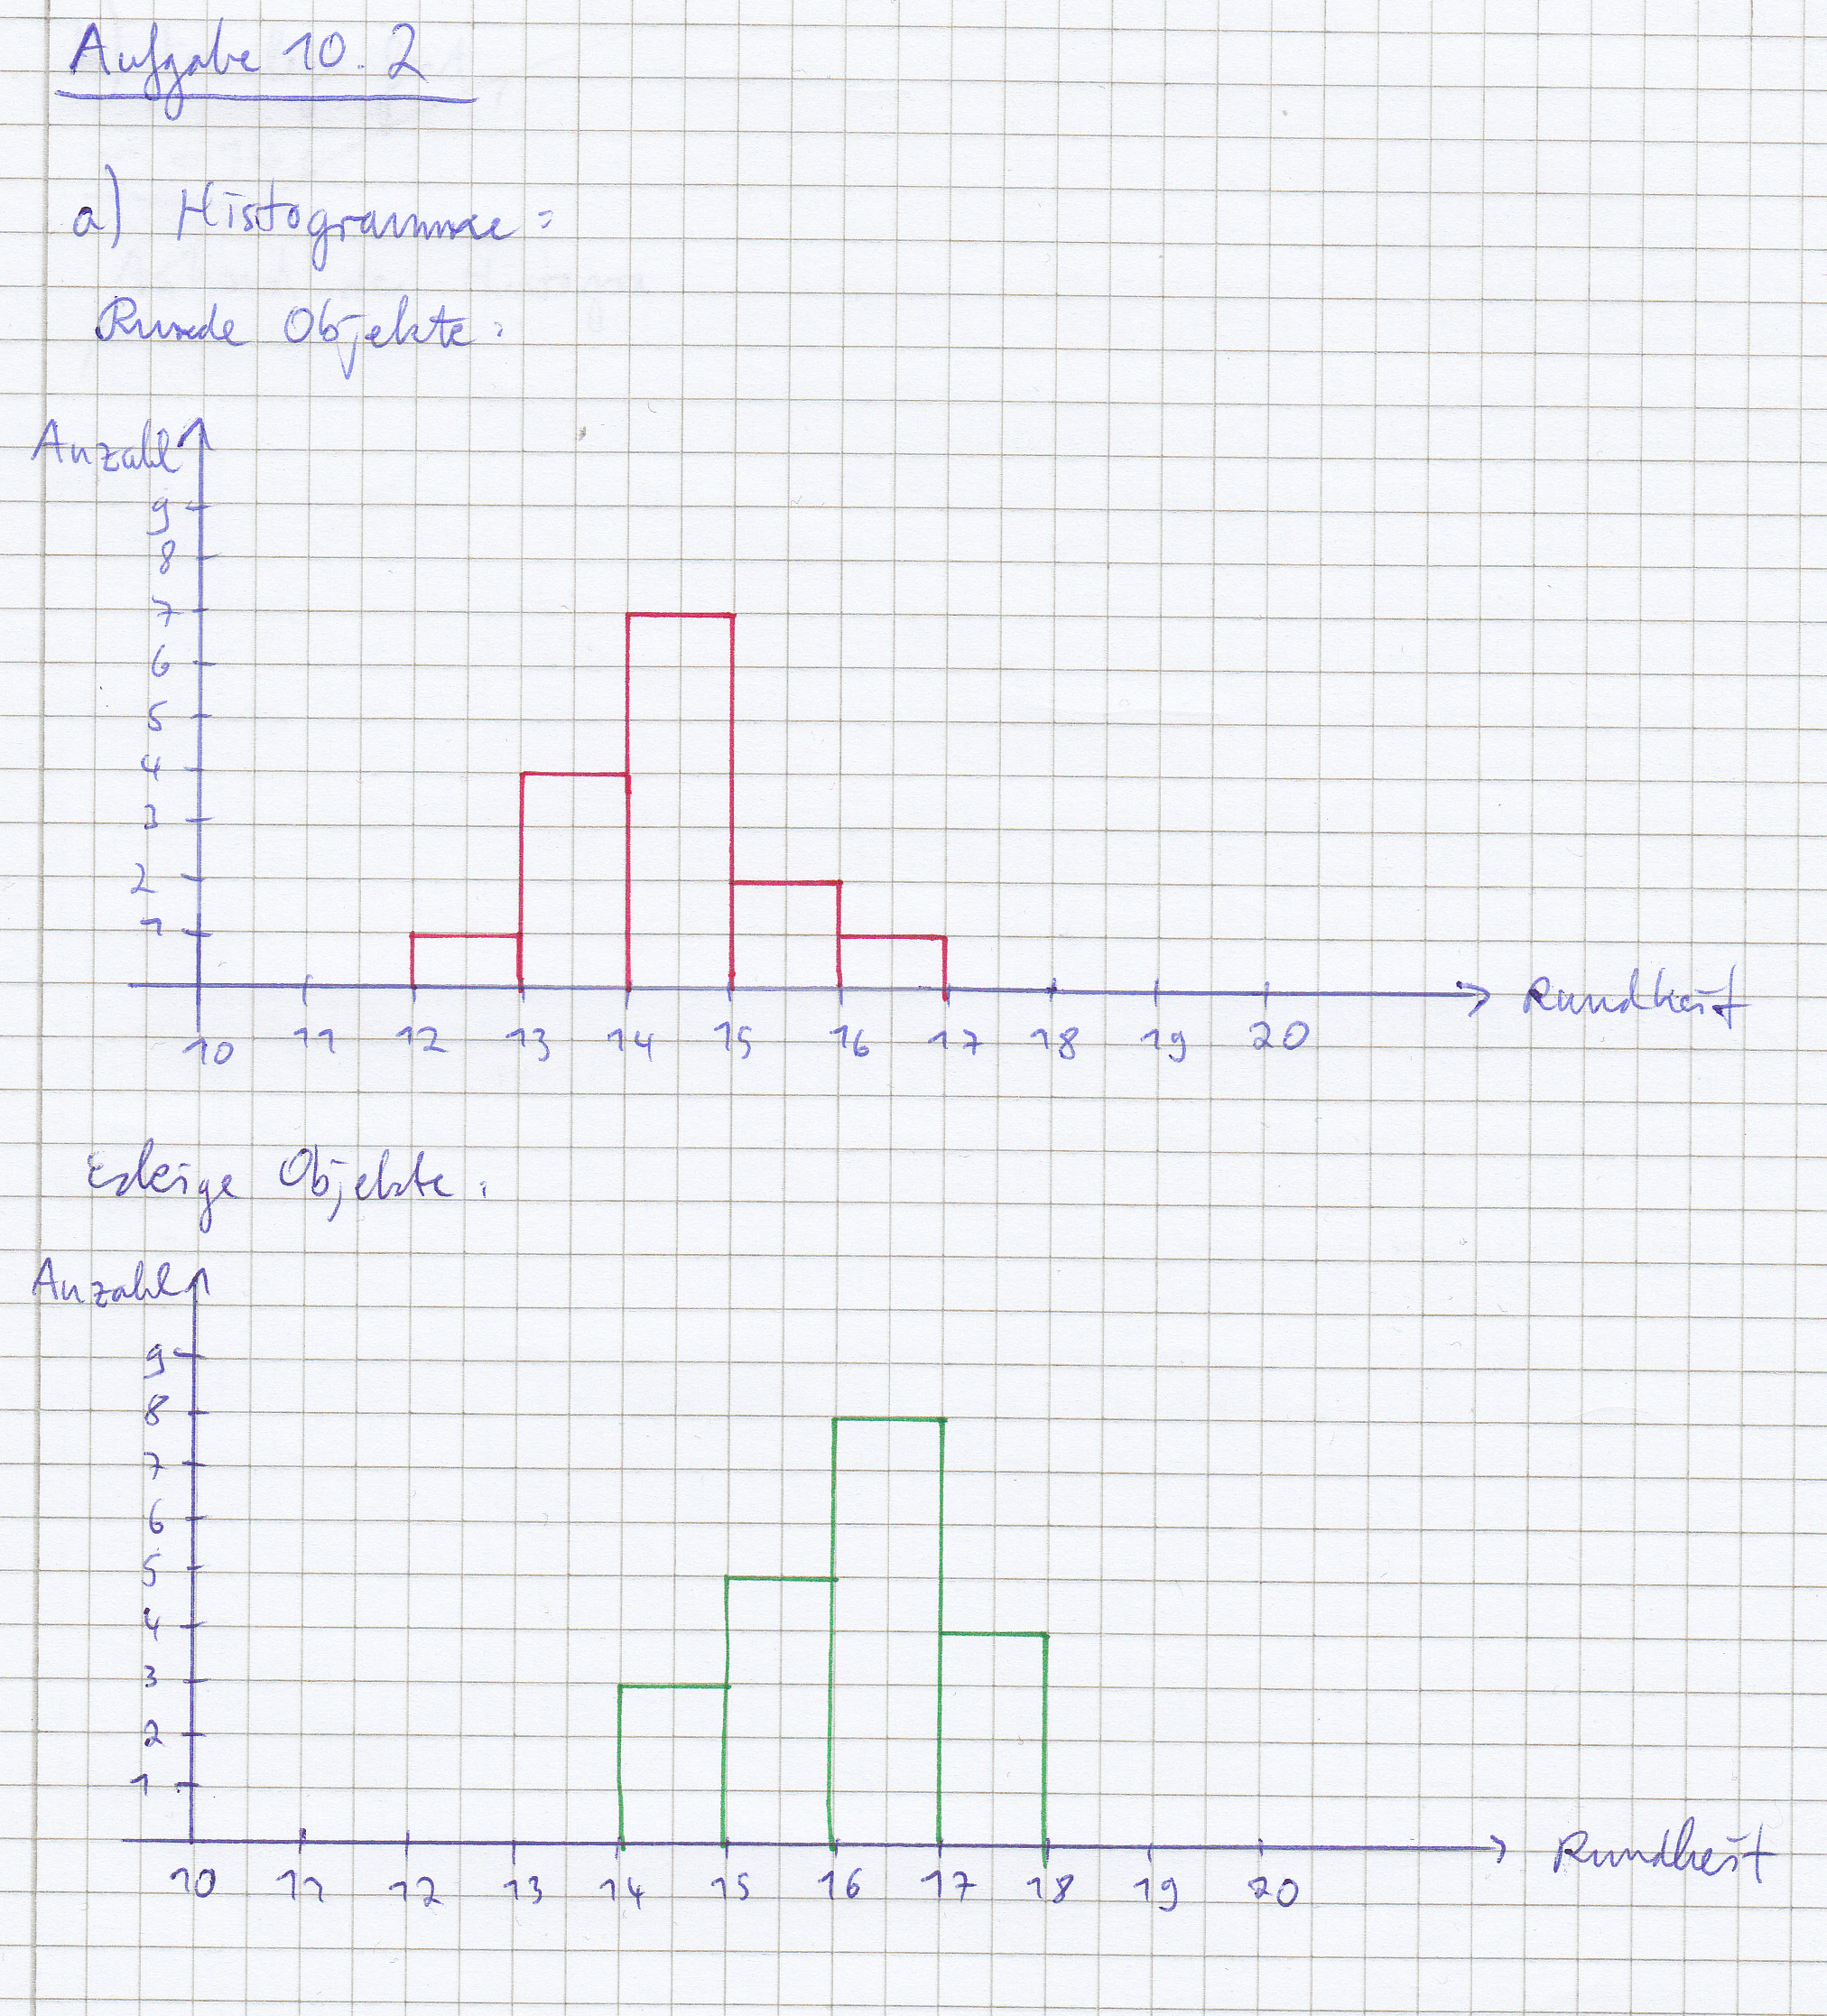
\includegraphics{Histogramme.jpg}

\newpage

\subsection*{b)}

Ich lege fest, dass die Klasse ,,Positive`` den runden Objekten, und die Klasse ,,Negative`` den eckigen Objekten 
entsprechen soll. 

Dann ergeben sich folgende Werte (die man aus den Histogrammen auslesen kann):

\subsubsection*{\underline{$\tau = 14$}}

\[ t_p = 5, f_n = 10, t_n = 20, f_p = 0 \]

Daraus ergeben sich die TPR und die FPR:

\[ TPR = \frac{t_p}{t_p + f_n} = \frac{5}{15} = \frac{1}{3} \approx 0.333 = 33.3 \% \]

\[ FPR = \frac{f_p}{t_n + f_p} = \frac{0}{20} = 0 = 0 \% \]

\subsubsection*{\underline{$\tau = 17$}}

Hier ergeben sich folgende Werte:

\[ t_p = 15, f_n = 0, t_n = 4, f_p = 16 \]

Daraus ergeben sich folgende TPR und FPR:

\[ TPR = \frac{t_p}{t_p + f_n} = \frac{15}{15} = 1 = 100 \% \]

\[ FPR = \frac{f_p}{t_n + f_p} = \frac{16}{20} = \frac{4}{5} = 0.8 = 80 \% \]

\subsection*{c)}

Es muss gelten: $f_p = f_n$. 

Diese Gleichheit ergibt sich gerade zum Beispiel bei $\tau = 14.95$. Hier gilt gerade, 
wie man aus der Liste der Rundheitswerte ablesen kann, dass:
$f_p = f_n = 3$. 

Au�erdem gilt f�r dieses $\tau$:
$t_p = 12, t_n = 17$. 

Damit ergeben sich folgende TPR und FPR:

\[ TPR = \frac{t_p}{t_p + f_n} = \frac{12}{15} = \frac{4}{5} = 0.8 = 80 \% \]

\[ FPR = \frac{f_p}{t_n + f_p} = \frac{3}{20} = 0.15 = 15 \% \]

Die Klassifikationsrate f�r dieses $\tau$ betr�gt 
$\frac{t_p+t_n}{t_p+t_n+f_p+f_n} = \frac{29}{35} \approx 0.829 = 82.9 \% $. 
Die Fehlklassifikationsrate betr�gt $\frac{f_p+f_n}{t_p+t_n+f_p+f_n} = \frac{6}{35} \approx 0.171 = 17.1 \% $. 

Die Skizze der ROC-Kurve befindet sich auf der folgenden Seite. 

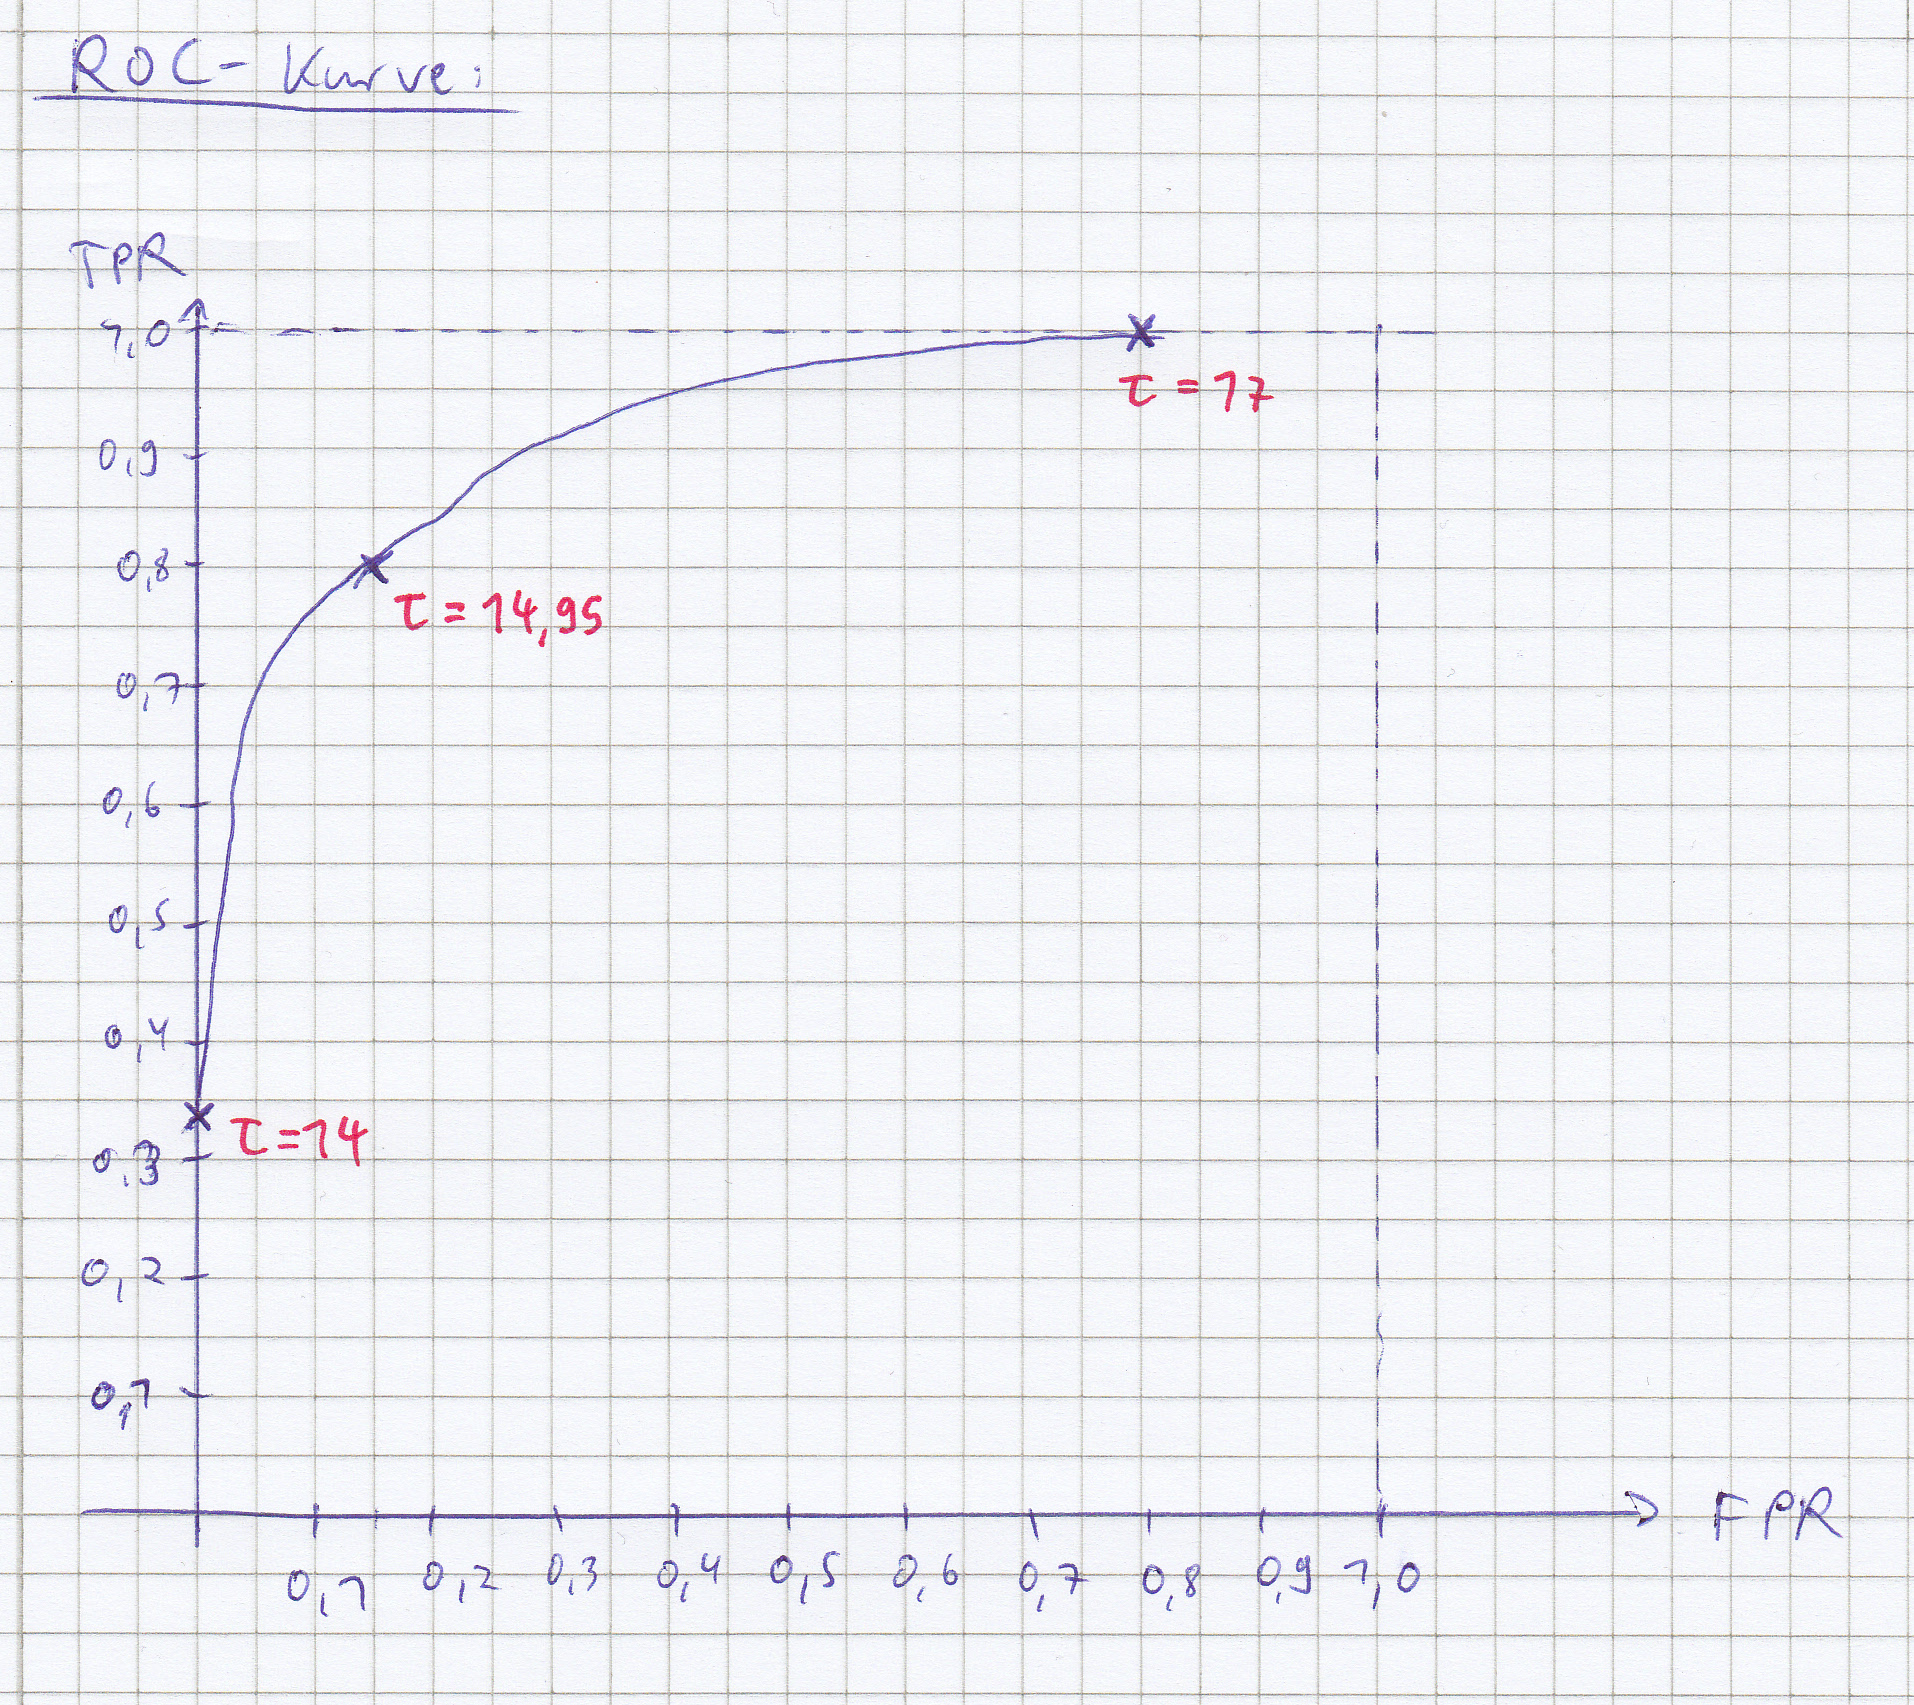
\includegraphics{ROC-Kurve.jpg}

\end{document}
